\chapter{Implementation}

\section{Hosting and Server Management}

The VPS we rented comes ready with a lot of tools to manage the server, is fully prepared for hosting,
is accessible via SSH and has a web-based control panel for managing the server.

After installing the .NET 8 runtime the process of running a .NET application was as simple as transfering the program via SFTP
and inputting 'dotnet Afantazie.dll' into the terminal.
Deploying the frontend required only copying the files to the necessary directory in the server filesystem.
DNS and SSL certificates got set-up in a mouse click in provided server-management.

The greatest challenge when hosting the application came with setting up reverse-proxy server (although that was mostly due to our inexperience with the technology).
Two provided reverse proxy server technologies were the default Apache and NginX.
After a short research through forums we decided to make the switch to NginX as it is more modern alternative to Apache and can have performance benefits.
If needed we could always switch back Apache without much hassle.

The provided template for the NginX configuration was a good starting point but in order to make the
application functional we had to make a few additions to the afantazie.cz.conf file:
\begin{itemize}
    \item Reroute the api requests to the backend
    \item Set up redirection from http to https
    \item Force the server to always provide new version of meta.json file used for cache busting (see Cache Busting section below)
\end{itemize}

With that the server was set up to host the database, backend and frontend.

\section{Database}

The database of Aphantasia is composed of just three tables:
\begin{itemize}
    \item \textbf{Users} - holds the user data
    \item \textbf{Thoughts} - holds the thought data
    \item \textbf{ThoughtReferences} - holds the links between the thoughts
\end{itemize}

A diagram of the database schema can be seen in figure \ref{obr:afantazie_database_schema}.

\begin{figure}[p]\centering
    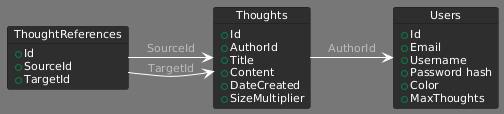
\includegraphics[width=90mm]{img/afantazie_database_schema.png}
    \caption{Aphantasia Database schema}
    \label{obr:afantazie_database_schema}
\end{figure}


\section{Backend}
The backend of the chat application is an ASP.NET application written in C\#.
We decided to develop architectural design early on and it paid off as development of later features was much easier. 
The initial architectural blueprint remained mostly unchanged up until the end of the project.

The solution of the backend consists of 19 projects implementing the backend to Aphantasia and one project for secondary tools (see chapter 6 - Afantazie.Tools for more details). 

The backend projects are divided into four directories (forming conceptual layers):
\begin{itemize}
    \item \textbf{Presentation}
    \item \textbf{Service}
    \item \textbf{Core} 
    \item \textbf{Data}
\end{itemize}

There is also one project outside of these layers that serves to Bootstrap the application and set up \gls{dependency_injection}.
In figure \ref{obr:afantazie_backend_architecture} you can see the architecture of the backend with its dependencies.

This division is loosely based on Onion architecture \cite{onion_architecture}. Notice that the Presentation layer doesn't directly depend on the Service layer.
Instead it depends on Service Interface layer and the actual implementation is injected at runtime.
This allows for clean separation of concerns, makes the code more testable and allows for easy swapping of implementations.

\begin{figure}[p]\centering
    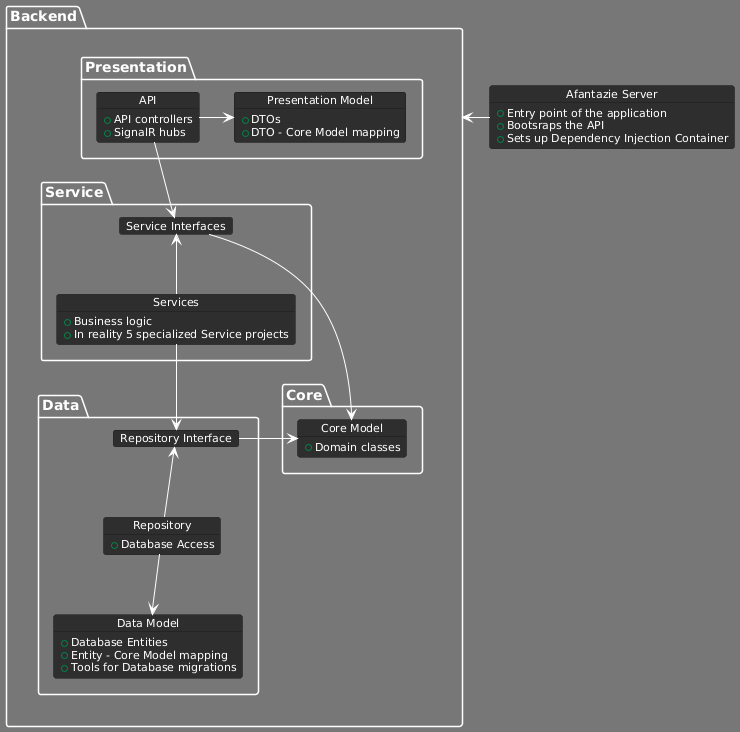
\includegraphics[width=140mm]{img/backend_architecture.png}
    \caption{Aphantasia Backend Architecture}
    \label{obr:afantazie_backend_architecture}
\end{figure}

Let us now take a look at the individual layers.

\subsection*{Presentation layer}
The Presentation layer sits in the outermost layer of the application and is responsible for handling HTTP requests and responses.
It contains two projects - \textbf{Api} and \textbf{Model}.

Api holds Api controllers implemented using Asp.NET Core MVC.
The controllers and signalR hubs only handle incomming traffic and  
for handling \gls{business_logic} they call the appropriate service in the Service layer.

The Presentation Model contains definitions for the data transfer objects (DTOs).
These objects are used to transfer data between the client and the server.

\subsection*{Service layer}
The Service contains the \gls{business_logic} of Aphantaisa.
It is set of 5 projects (and their respective interfaces):
\begin{itemize}
    \item \textbf{Auth} - handles user registration, login and JWT token generation
    \item \textbf{Chat} - handles the chat functionality
    \item \textbf{Site Activity} - handles the real-time stats of the site (such as the number of users online)
    \item \textbf{Thoughts} - handles the creation and retrieval of thoughts
    \item \textbf{UserSettings} - handles the user settings (such as selected color or on-screen thoughts limit)
\end{itemize}

\subsection*{Core layer}
The Core contains three projects:
\begin{itemize}
    \item \textbf{Core Model} - contains the core model of the application used in Repository and Service interfaces as arguments
    \item \textbf{Localization} - contains the localization resources for the application
    \item \textbf{Constants} - contains constants (currently only the default on-screen thoughts limit for newly registered users)
\end{itemize}

This layer sits in the midle of the application dependency wise and is used by both the Service and Data layers.

\subsection*{Data layer}
The Data layer is called by services to access the database using Entity Framework Core.
It contains Repository project and its interface.
The Repository project is responsible for handling the database queries and updates.

\subsection*{AfantazieServer project}
Since the application is using \gls{dependency_injection}
we cannot put its entry point inside any of the projects mentioned above without breaking the principles of the Onion architecture \cite{onion_architecture}
If we for example wanted to run the API by setting setting the Presentation.Api as startup project we would have to add
references to Service layer and Data layer to add their classes to \gls{dependency_injection} container and thus break the separation of concerns.

Instead we created a separate project that serves as the entry point to the application.
It is responsible for all the setup and configuration of the application which includes but is not limited to:
\begin{itemize}
    \item Configuration files 
    \item Dependency injection setup
    \item CORS setup (Cross-Origin Resource Sharing)
    \item Logging setup
\end{itemize}

Note that not all of these setups are done in the AfantazieServer project itself.
Instead they are defined inside their respective projects and are only called from the AfantazieServer project.
For example, AfantazieServer project calls AddDataModule() method from the Data project
which then registers the Data module with all its responsibilities allowing to swap modules for different implementation if needed.

\subsection*{Models}
You might have noticed that we use three different models in the application.
That is not an oversight as each model serves different purspose:
\begin{itemize}
    \item \textbf{Presentation Model} - DTOs used for transmition between client and server
    (client has to implement the exact same model to be able to communicate with the server)
    \item \textbf{Data Model} - Entities correspond to Database tables
    (which is created \gls{code_first} from the entities by Entity Framework)
    \item \textbf{Core Model} - Serves as an intemediary between the Presentation and Data models.
    Business logic should be implemented in the Service layer using this model.
\end{itemize}

Both Repository and Service interfaces use the Core Model as arguments and return values.
This means that the Service layer is not dependent on neither the Entities or the DTOs,
but it also requires mapping between the Core Model and the Data Model.
For mapping we used Mapster library inside Data and Presentation Model projects.

\section{Frontend}
The frontend of the application is a React web application written in Typescript.

As a warmup before graph rendering we built a small chat application in React.
The goal was to initialize the architecture and implement \gls{auth_x_y},
real-time server-client communication and routing with a few pages:
\begin{itemize}
    \item Home page
    \item Login page
    \item Registration page
    \item Chat page
    \item About page
\end{itemize}

We also styled the application using plain css and while the resulting design is not the most visually appealing,
it is functional and serves as a good starting point for the development of the graph view.

\subsection{Cache busting}
Browsers routinely cache files to speed up the loading of websites.
This is a good thing as it reduces the load on the server and speeds up the user experience.
However when the website is in active development and the files are changing frequently the cache can become a problem.
Users might not see the changes made to the website because the browser is loading the old cached version of the file.
The techniques solving this problem are called Cache busting. We used a react library called React cache buster to resolve this issue.

At first we had no success with the library as it was not working as expected.
The reason, as we found out, was that the library uses a meta.json file to store the version of the application.
Client then checks the version of the application and if it is different from the version in the meta.json file
it forcefully reloads the page to get the new version of the application.

The problem was that nginX was caching the meta.json file and the client was not getting the new version of the file.
Instead it was getting response with 304 status code (not modified).
We solved this by adding a directive to the nginX configuration file that forces the server to always provide a new version of the file.

\subsection{Server-Client communication}
For the chat application we tried to use \gls{websockets} for real time communication.
While we did manage to get this approach working, we did not like the developer experience.

SignalR is a library that simplifies the process of setting up websockets and provides a nice API for server-client communication.
It's available for both .NET and Javascript and is easy to set up, with much less boilerplate code than using websockets directly.

SignalR uses so called hubs to communicate between server and client which automatically handle
the connection and disconnection of clients.

We implemented two hubs - chatHub and statshub, with the former being used for chat messages while on the chat page
and the latter used across the entire application to keep track and display the number of users online on the homepage.

This feature can be exploited further, for example to inform the client that new thoughts were created.

\section{Small graph vizualization}
Small graph implementation required only two things - rendering and focres simulation.
As mentioned previously, we decided to render the graph using Pixi.js and implement our proprietary \gls{FDL}.

To integrate Pixi.js into the React application we first followed the official documentation \cite{pixijs_official_react_guide}.
We were not happy with the result as the pixi/react components were hard to work with programmatically.

So instead we used guide by Adam Emery \cite{pixijs_adam_emery_guide} to integrate Pixi.js into the React application.
His approach is different in that it only uses the Stage component from the pixi/react library
and the rest of the Pixi.js code is written in plain javascript (in our case typescript).
This allows us to better control the Pixi.js code and use the full potential of the library instead of using the pixi/react wrapper.

After implementing a simple node and edges rendering, we quickly hit a roadblock with massive \glspl{memory_leak}.
As we found out we were instantiating new Pixi.js objects every time the graph was updated.
To mitigate this issue we created an interface - RenderedThought - that holds the Pixi.js objects for each thought (the Title text and the Circle graphics).

The RenderedThought interface remained to the end of the development and we incrementaly added more properties to it as we needed them.
It contains all the properties that are needed to render the thought on the screen and to interact with it.
For example, each rendered thought has a boolean property 'held' which is used to determine if the thought is currently being dragged by the user.

Once we were able to render nodes and edges, we created a simple force directed layout algorithm with two forces - pull connected and push unconnected.
At this point we had an application with comparable graph view to obsidian (figure \ref{obr:afantazie_selfie}).

In figure \ref{obr:afantazie_cithep_3k} you can see again the first 3000 nodes of the citHep dataset now visiaulised using Aphantasia.
With this many nodes on screen the application lagged a lot. Although it remained somewhat usable.

\begin{figure}[p]\centering
    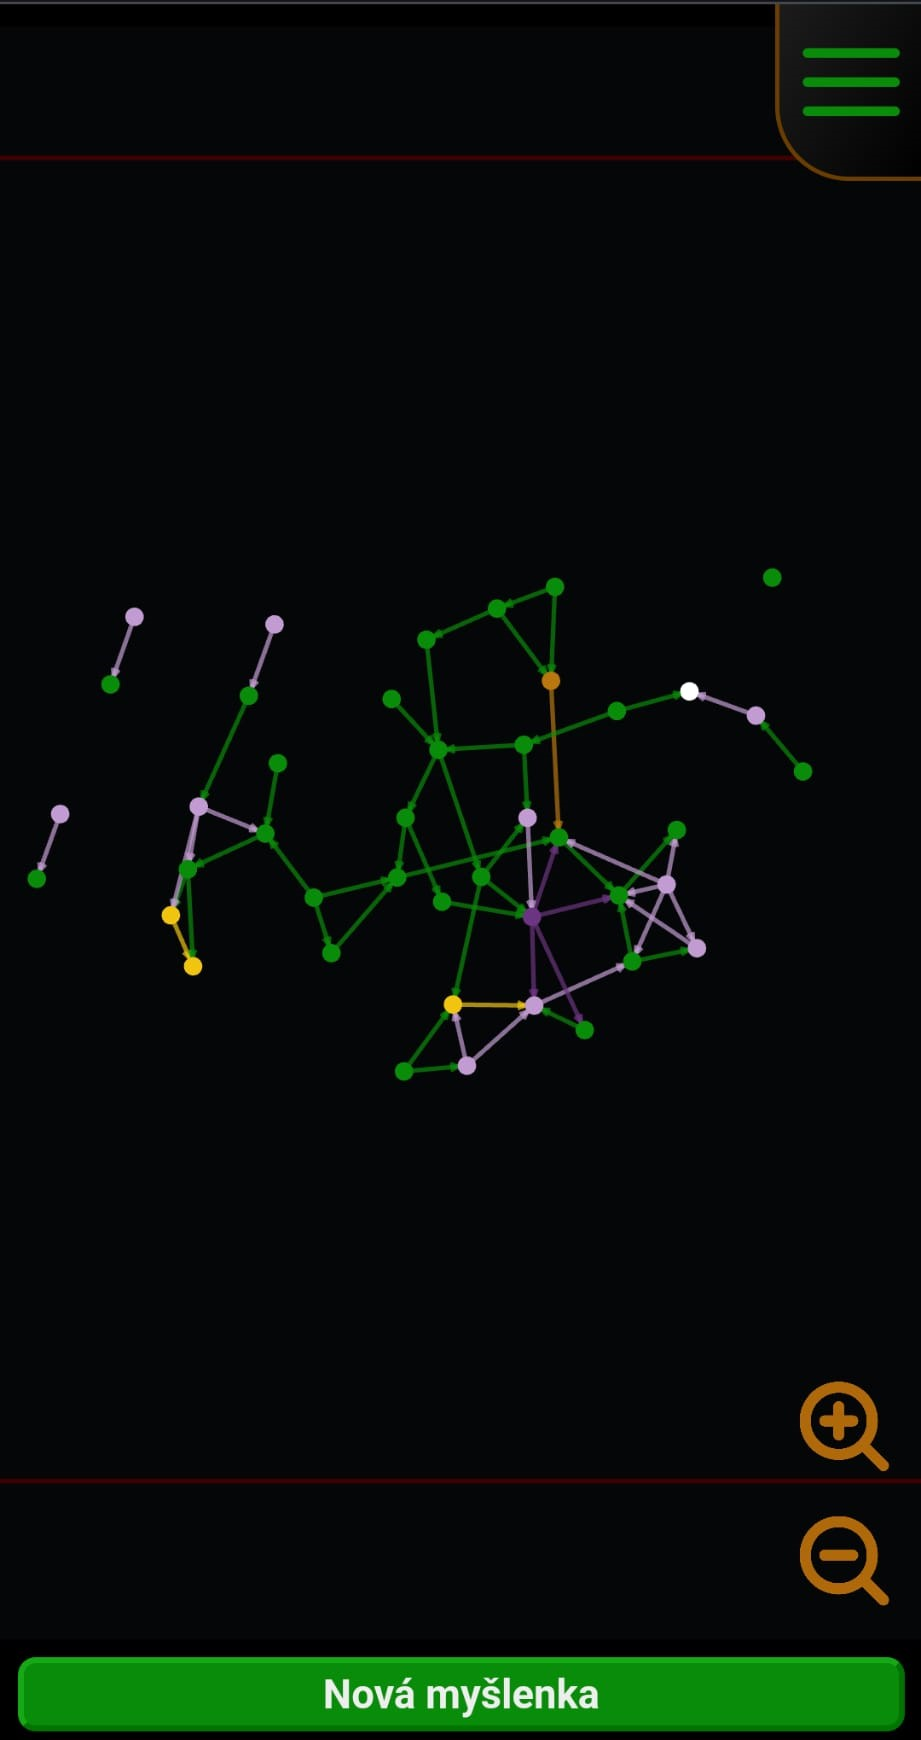
\includegraphics[width=100mm, keepaspectratio]{img/afantazie_first_stage_done.jpg}
    \caption{Aphantasia graph view at the end of the small graph development stage}
    \label{obr:afantazie_selfie}
\end{figure}

\begin{figure}[p]\centering
    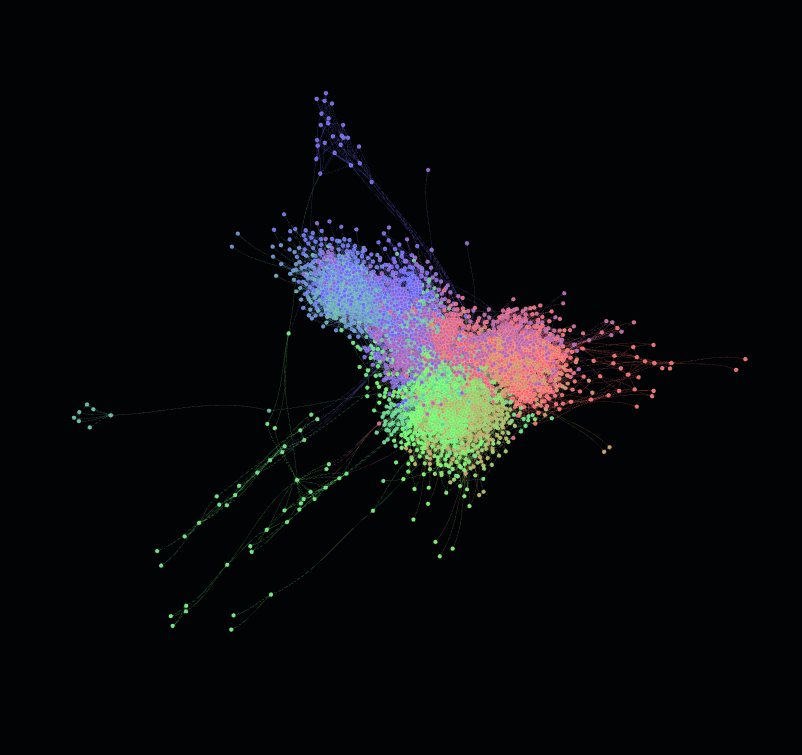
\includegraphics[width=140mm, keepaspectratio]{img/Afantazie_cithep_3000.png}
    \caption{The first 3000 nodes of the CitHep dataset visualized in Aphantasia (before big graph solution)}
    \label{obr:afantazie_cithep_3k}
\end{figure}

\section{Big graph visualization}

\subsection*{State management}

So far we used React states and contexts to hold and manage the information of the graph context.
This worked for simple small graph approach but we were not happy with this approach once the context started to become more complicated.

A solution we used is a react library called Zustand \cite{zustand_homepage}.
This library allows minimal state setup that is compatible with external (meaning outside react) code.

We had to implement time slider and that provided a suprisingly nice way of handling big graphs.

\subsection*{Dynamic loading}
At the beginning of the development we used one endpoint for all the data at once.
That worked until around 500 thoughts after which the loading time became quite noticable. 

The obvious solution was to load only a subset of the data at a time. We implemented this in several ways:
\begin{itemize}
    \item \textbf{Temporal API endpoints} - Client requests new subset of nodes in a form of "beforeId / afterId / aroundId".
    Thanks to ascending ID increment approach translates to chronological order of the nodes.
    When time window exceeds the currently loaded data it gets updated with missing nodes from the relative past or future.
    \item \textbf{Neighborhood API endpoints} - Breadth-first search starting in given node up to given depth. is used to implement graph walk.
\end{itemize}

This approach worked not just as an optimization technique but we ended up building our big graph handling on it.
We will look at the result in the next chapter.

\section{Frontend architecture}

The frontend architecture is much less clear-cut than the backend
but we tried to visualise the relationship between the main surce code files in figure
\ref{obr:afantazie_frontend_architecture}.
All of the graph-related code sits inside the src/pages/graph directory of the AfantazieWeb project
and the containers in the diagram correspond to the folder structure.

\begin{figure}[p]\centering
    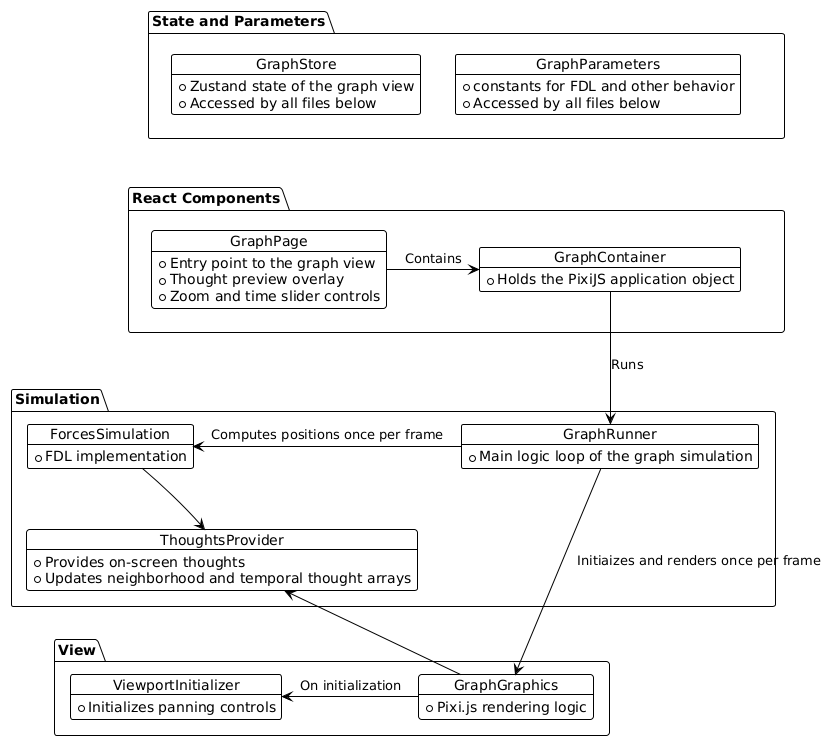
\includegraphics[width=140mm, keepaspectratio]{img/afantazie_frontend_architecture.png}
    \caption{The frontend architecture of Aphantasia}
    \label{obr:afantazie_frontend_architecture}
\end{figure}

Let's look at the individual parts of the frontend architecture:
\subsection*{React}
\textbf{Graph Page} contains the UI elements of the graph view:
\begin{itemize}
    \item Content preview
    \item Controls (zoom and time slider)
    \item Time window date label
    \item New thought button
\end{itemize}
It also handles much of the initialization logic such as getting the thought ID from the URL and fetching the appropriate data
(either latest or around the requested thought).

\textbf{Graph Container}
This component is the bridge between React and Pixi.js code. It calls the run() method of the \textbf{Graph Runer}.

\subsection*{Simulation}
In the Simulation directory we find three files:
\begin{itemize}
    \item \textbf{Graph Runner} - Contains the main logic loop of the graph simulation.
    Its run() method is called by the Graph Container and it initializes the graphics,
    runs the render function and the simulation functions.
    \item \textbf{Forces Simulation} - Custom FDA implementation.
    \item \textbf{ThoughtsProvider} - Responsible for providing the temporal and neighborhood thoughts as well as
    fetching data from backend based on time window position and graph walk state.
\end{itemize}

\subsection*{Graphics}
This directory contains two files:
\begin{itemize}
    \item \textbf{Graphics} - Contains the initializeGraphics() method which returns a callback function render()
    called by the Graph Runner every loop.
    \item \textbf{ViewportInitializer} - Contains the addDraggableViewport() method
    which sets up the viewport for the graph. 
\end{itemize}

\subsection*{State and parameters}
Here we find two files:
\begin{itemize}
    \item \textbf{Graph Store} - Zustand store for the graph state.
    \item \textbf{Graph Parameters} - Constants used in the graph view, \gls{FDL} and other behavior.
\end{itemize}

